\documentclass{article}

\usepackage{tikz}
\usetikzlibrary{arrows,calc,decorations.markings}

\begin{document}
\pgfarrowsdeclarecombine{dimarrow}{dimarrow}{latex}{latex}{}{}
\def\Dimline[#1][#2][#3]{
        \draw[|-|,
        decoration={markings, % switch on markings
                mark=at position 0 with {\arrowreversed[scale=0.5]{dimarrow}};,
                mark=at position .5 with {\node[gray] at (0,0.25) {\tiny{#3}};},
                mark=at position 1 with {\arrow[scale=0.5]{dimarrow}};,
            },
        postaction=decorate] #1 -- #2 ;
}

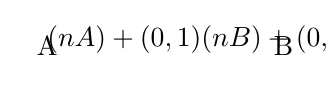
\begin{tikzpicture}

    \node at (0,0) (nA) {A};
    \node at (3,0) (nB) {B};
    \Dimline[($(nA)+(0,1)$)][($(nB)+(0,1)$)]['test'] ;

\end{tikzpicture}

\end{document}